\documentclass[runningheads]{llncs}

\usepackage[T1]{fontenc}
\usepackage[utf8]{inputenc}
\usepackage{lmodern}
\usepackage{graphicx}
\usepackage{amsmath,amssymb}
\usepackage{booktabs}
\usepackage{multirow}
\usepackage{xcolor}
\usepackage{algorithm}
\usepackage{algpseudocode}
\usepackage{tikz}
\usetikzlibrary{arrows.meta,positioning,fit,calc}
\usepackage[hidelinks]{hyperref}

\newcommand{\NOA}{\textsc{NoAction}}
\newcommand{\TA}{\textsc{ThreadAdjust}}
\newcommand{\RB}{\textsc{Rebalance}}
\newcommand{\RP}{\textsc{Repartition}}
% placeholder for a number that must come from results/ (none may remain at submission)
\newcommand{\RES}[1]{\textbf{\textcolor{red}{[#1]}}}
% every number quoted in the text, generated by experiments/numbers.py
% generated by experiments/numbers.py -- do not edit
\newcommand{\CEacc}{0.727}
\newcommand{\CEregret}{0.65}
\newcommand{\CEregretStd}{0.05}
\newcommand{\CalMape}{12}
\newcommand{\CalPoints}{240}
\newcommand{\CalRtwo}{0.96}
\newcommand{\CtrlGSAGE}{2.6}
\newcommand{\CtrlMPC}{47.2}
\newcommand{\EOneCoraAcgrMs}{2}
\newcommand{\EOneCoraHashCutRed}{69}
\newcommand{\EOneCoraHashLPRed}{59}
\newcommand{\EOneCoraLDGCutRed}{37}
\newcommand{\EOneCoraLDGLPRed}{26}
\newcommand{\EOneCoraMetisCVRed}{3.9}
\newcommand{\EOneCoraMetisCutRed}{1.2}
\newcommand{\EOneCoraMetisMs}{6}
\newcommand{\EOneMathAcgrMs}{121}
\newcommand{\EOneMathHashCutRed}{16}
\newcommand{\EOneMathHashLPRed}{16}
\newcommand{\EOneMathLDGCutRed}{2}
\newcommand{\EOneMathLDGLPRed}{3}
\newcommand{\EOneMathMetisCVRed}{7.5}
\newcommand{\EOneMathMetisCutRed}{3.8}
\newcommand{\EOneMathMetisMs}{158}
\newcommand{\EOnePubAcgrMs}{22}
\newcommand{\EOnePubHashCutRed}{58}
\newcommand{\EOnePubHashLPRed}{52}
\newcommand{\EOnePubLDGCutRed}{41}
\newcommand{\EOnePubLDGLPRed}{32}
\newcommand{\EOnePubMetisCVRed}{4.1}
\newcommand{\EOnePubMetisCutRed}{-0.4}
\newcommand{\EOnePubMetisMs}{56}
\newcommand{\FasterAlwaysTA}{9}
\newcommand{\FasterGSAGE}{9}
\newcommand{\FasterMLP}{9}
\newcommand{\FasterThreshold}{9}
\newcommand{\GSFOne}{0.47}
\newcommand{\GSPredRB}{10}
\newcommand{\GSPredRP}{0}
\newcommand{\GSRBprec}{47}
\newcommand{\GSRBrecall}{50}
\newcommand{\GSRPasRB}{40}
\newcommand{\GSacc}{0.720}
\newcommand{\GSregret}{0.69}
\newcommand{\GSregretStd}{0.07}
\newcommand{\LabelNO}{63.3}
\newcommand{\LabelRB}{8.6}
\newcommand{\LabelRP}{4.3}
\newcommand{\LabelTA}{23.8}
\newcommand{\MLPFOne}{0.45}
\newcommand{\MLPPredRB}{8}
\newcommand{\MLPPredRP}{0}
\newcommand{\MLPRBprec}{45}
\newcommand{\MLPRBrecall}{41}
\newcommand{\MLPRPasRB}{37}
\newcommand{\MLPacc}{0.720}
\newcommand{\MLPregret}{0.69}
\newcommand{\MLPregretStd}{0.02}
\newcommand{\MathActive}{49}
\newcommand{\MathInteractions}{390{,}441}
\newcommand{\MathRBGSAGE}{0}
\newcommand{\MathRBOracle}{50}
\newcommand{\MathRPGSAGE}{0}
\newcommand{\MathRPOracle}{13}
\newcommand{\MathYears}{6.4}
\newcommand{\NOregret}{1.20}
\newcommand{\NumSamples}{7,200}
\newcommand{\NumScenarios}{12}
\newcommand{\NumTest}{1,088}
\newcommand{\NumTestGraphs}{68}
\newcommand{\PubActive}{9}
\newcommand{\RBallregret}{8.51}
\newcommand{\RPallregret}{17.93}
\newcommand{\ReconfMs}{1.4}
\newcommand{\RobAlwaysACGRMax}{46.1}
\newcommand{\RobAlwaysACGRMean}{20.6}
\newcommand{\RobAlwaysACGRWins}{0}
\newcommand{\RobAlwaysTAMax}{10.7}
\newcommand{\RobAlwaysTAMean}{3.0}
\newcommand{\RobAlwaysTAWins}{6}
\newcommand{\RobGSAGEMax}{11.0}
\newcommand{\RobGSAGEMean}{4.3}
\newcommand{\RobGSAGEWins}{0}
\newcommand{\RobMLPMax}{10.9}
\newcommand{\RobMLPMean}{4.1}
\newcommand{\RobMLPWins}{0}
\newcommand{\RobMPCMax}{253.7}
\newcommand{\RobMPCMean}{94.4}
\newcommand{\RobMPCWins}{0}
\newcommand{\RobOracleGap}{14}
\newcommand{\RobOracleMax}{5.6}
\newcommand{\RobOracleMean}{0.1}
\newcommand{\RobOracleWins}{0}
\newcommand{\RobPMETISMax}{50.0}
\newcommand{\RobPMETISMean}{11.2}
\newcommand{\RobPMETISWins}{6}
\newcommand{\RobStaticMax}{24.1}
\newcommand{\RobStaticMean}{8.3}
\newcommand{\RobStaticWins}{0}
\newcommand{\RobThresholdMax}{10.8}
\newcommand{\RobThresholdMean}{3.3}
\newcommand{\RobThresholdWins}{0}
\newcommand{\SigFasterAlwaysTA}{6}
\newcommand{\SigFasterGSAGE}{5}
\newcommand{\SigFasterMLP}{5}
\newcommand{\SigFasterThreshold}{6}
\newcommand{\SpMathEightOneAlwaysACGR}{0.96}
\newcommand{\SpMathEightOneAlwaysTA}{1.00}
\newcommand{\SpMathEightOneGSAGE}{1.00}
\newcommand{\SpMathEightOneMLP}{1.00}
\newcommand{\SpMathEightOneMPC}{0.94}
\newcommand{\SpMathEightOneOracle}{1.07}
\newcommand{\SpMathEightOnePMETIS}{1.05}
\newcommand{\SpMathEightOneStatic}{1.00}
\newcommand{\SpMathEightOneThreshold}{1.00}
\newcommand{\SpMathEightSmAlwaysACGR}{0.84}
\newcommand{\SpMathEightSmAlwaysTA}{0.98}
\newcommand{\SpMathEightSmGSAGE}{0.99}
\newcommand{\SpMathEightSmMLP}{0.99}
\newcommand{\SpMathEightSmMPC}{0.59}
\newcommand{\SpMathEightSmOracle}{1.03}
\newcommand{\SpMathEightSmPMETIS}{1.03}
\newcommand{\SpMathEightSmStatic}{1.00}
\newcommand{\SpMathEightSmThreshold}{0.99}
\newcommand{\SpMathEightTenAlwaysACGR}{0.89}
\newcommand{\SpMathEightTenAlwaysTA}{0.99}
\newcommand{\SpMathEightTenGSAGE}{0.99}
\newcommand{\SpMathEightTenMLP}{0.99}
\newcommand{\SpMathEightTenMPC}{0.71}
\newcommand{\SpMathEightTenOracle}{1.03}
\newcommand{\SpMathEightTenPMETIS}{1.03}
\newcommand{\SpMathEightTenStatic}{1.00}
\newcommand{\SpMathEightTenThreshold}{0.99}
\newcommand{\SpMathFourOneAlwaysACGR}{1.03}
\newcommand{\SpMathFourOneAlwaysTA}{1.02}
\newcommand{\SpMathFourOneGSAGE}{1.01}
\newcommand{\SpMathFourOneMLP}{1.01}
\newcommand{\SpMathFourOneMPC}{0.97}
\newcommand{\SpMathFourOneOracle}{1.16}
\newcommand{\SpMathFourOnePMETIS}{1.13}
\newcommand{\SpMathFourOneStatic}{1.00}
\newcommand{\SpMathFourOneThreshold}{1.02}
\newcommand{\SpMathFourSmAlwaysACGR}{0.96}
\newcommand{\SpMathFourSmAlwaysTA}{1.07}
\newcommand{\SpMathFourSmGSAGE}{1.04}
\newcommand{\SpMathFourSmMLP}{1.06}
\newcommand{\SpMathFourSmMPC}{0.63}
\newcommand{\SpMathFourSmOracle}{1.14}
\newcommand{\SpMathFourSmPMETIS}{1.13}
\newcommand{\SpMathFourSmStatic}{1.00}
\newcommand{\SpMathFourSmThreshold}{1.06}
\newcommand{\SpMathFourTenAlwaysACGR}{0.98}
\newcommand{\SpMathFourTenAlwaysTA}{1.05}
\newcommand{\SpMathFourTenGSAGE}{1.04}
\newcommand{\SpMathFourTenMLP}{1.04}
\newcommand{\SpMathFourTenMPC}{0.74}
\newcommand{\SpMathFourTenOracle}{1.13}
\newcommand{\SpMathFourTenPMETIS}{1.12}
\newcommand{\SpMathFourTenStatic}{1.00}
\newcommand{\SpMathFourTenThreshold}{1.05}
\newcommand{\SpPubEightOneAlwaysACGR}{0.96}
\newcommand{\SpPubEightOneAlwaysTA}{1.04}
\newcommand{\SpPubEightOneGSAGE}{1.03}
\newcommand{\SpPubEightOneMLP}{1.03}
\newcommand{\SpPubEightOneMPC}{0.75}
\newcommand{\SpPubEightOneOracle}{1.06}
\newcommand{\SpPubEightOnePMETIS}{0.95}
\newcommand{\SpPubEightOneStatic}{1.00}
\newcommand{\SpPubEightOneThreshold}{1.04}
\newcommand{\SpPubEightSmAlwaysACGR}{0.85}
\newcommand{\SpPubEightSmAlwaysTA}{1.25}
\newcommand{\SpPubEightSmGSAGE}{1.20}
\newcommand{\SpPubEightSmMLP}{1.21}
\newcommand{\SpPubEightSmMPC}{0.35}
\newcommand{\SpPubEightSmOracle}{1.22}
\newcommand{\SpPubEightSmPMETIS}{0.84}
\newcommand{\SpPubEightSmStatic}{1.00}
\newcommand{\SpPubEightSmThreshold}{1.23}
\newcommand{\SpPubEightTenAlwaysACGR}{0.94}
\newcommand{\SpPubEightTenAlwaysTA}{1.09}
\newcommand{\SpPubEightTenGSAGE}{1.08}
\newcommand{\SpPubEightTenMLP}{1.08}
\newcommand{\SpPubEightTenMPC}{0.57}
\newcommand{\SpPubEightTenOracle}{1.08}
\newcommand{\SpPubEightTenPMETIS}{0.93}
\newcommand{\SpPubEightTenStatic}{1.00}
\newcommand{\SpPubEightTenThreshold}{1.08}
\newcommand{\SpPubFourOneAlwaysACGR}{0.83}
\newcommand{\SpPubFourOneAlwaysTA}{1.03}
\newcommand{\SpPubFourOneGSAGE}{1.01}
\newcommand{\SpPubFourOneMLP}{1.01}
\newcommand{\SpPubFourOneMPC}{0.56}
\newcommand{\SpPubFourOneOracle}{1.04}
\newcommand{\SpPubFourOnePMETIS}{0.89}
\newcommand{\SpPubFourOneStatic}{1.00}
\newcommand{\SpPubFourOneThreshold}{1.02}
\newcommand{\SpPubFourSmAlwaysACGR}{0.78}
\newcommand{\SpPubFourSmAlwaysTA}{1.08}
\newcommand{\SpPubFourSmGSAGE}{1.04}
\newcommand{\SpPubFourSmMLP}{1.04}
\newcommand{\SpPubFourSmMPC}{0.32}
\newcommand{\SpPubFourSmOracle}{1.02}
\newcommand{\SpPubFourSmPMETIS}{0.86}
\newcommand{\SpPubFourSmStatic}{1.00}
\newcommand{\SpPubFourSmThreshold}{1.07}
\newcommand{\SpPubFourTenAlwaysACGR}{0.83}
\newcommand{\SpPubFourTenAlwaysTA}{1.05}
\newcommand{\SpPubFourTenGSAGE}{1.03}
\newcommand{\SpPubFourTenMLP}{1.03}
\newcommand{\SpPubFourTenMPC}{0.42}
\newcommand{\SpPubFourTenOracle}{1.02}
\newcommand{\SpPubFourTenPMETIS}{0.90}
\newcommand{\SpPubFourTenStatic}{1.00}
\newcommand{\SpPubFourTenThreshold}{1.05}
\newcommand{\SpeedupMax}{6.6}
\newcommand{\SpeedupMaxThreads}{9}
\newcommand{\SpeedupSix}{4.9}
\newcommand{\SpeedupTwelve}{5.8}
\newcommand{\TAallregret}{1.16}
\newcommand{\THFOne}{0.31}
\newcommand{\THregret}{0.91}
\newcommand{\TotMathEightOneAlwaysACGR}{28.60}
\newcommand{\TotMathEightOneAlwaysTA}{27.54}
\newcommand{\TotMathEightOneGSAGE}{27.53}
\newcommand{\TotMathEightOneMLP}{27.53}
\newcommand{\TotMathEightOneMPC}{29.18}
\newcommand{\TotMathEightOneOracle}{25.59}
\newcommand{\TotMathEightOnePMETIS}{26.27}
\newcommand{\TotMathEightOneStatic}{27.46}
\newcommand{\TotMathEightOneThreshold}{27.50}
\newcommand{\TotMathEightSmAlwaysACGR}{5.91}
\newcommand{\TotMathEightSmAlwaysTA}{5.01}
\newcommand{\TotMathEightSmGSAGE}{5.00}
\newcommand{\TotMathEightSmMLP}{4.99}
\newcommand{\TotMathEightSmMPC}{8.33}
\newcommand{\TotMathEightSmOracle}{4.80}
\newcommand{\TotMathEightSmPMETIS}{4.79}
\newcommand{\TotMathEightSmStatic}{4.93}
\newcommand{\TotMathEightSmThreshold}{4.98}
\newcommand{\TotMathEightTenAlwaysACGR}{9.55}
\newcommand{\TotMathEightTenAlwaysTA}{8.61}
\newcommand{\TotMathEightTenGSAGE}{8.59}
\newcommand{\TotMathEightTenMLP}{8.58}
\newcommand{\TotMathEightTenMPC}{12.03}
\newcommand{\TotMathEightTenOracle}{8.26}
\newcommand{\TotMathEightTenPMETIS}{8.31}
\newcommand{\TotMathEightTenStatic}{8.53}
\newcommand{\TotMathEightTenThreshold}{8.57}
\newcommand{\TotMathFourOneAlwaysACGR}{16.99}
\newcommand{\TotMathFourOneAlwaysTA}{17.27}
\newcommand{\TotMathFourOneGSAGE}{17.32}
\newcommand{\TotMathFourOneMLP}{17.31}
\newcommand{\TotMathFourOneMPC}{18.08}
\newcommand{\TotMathFourOneOracle}{15.15}
\newcommand{\TotMathFourOnePMETIS}{15.61}
\newcommand{\TotMathFourOneStatic}{17.56}
\newcommand{\TotMathFourOneThreshold}{17.30}
\newcommand{\TotMathFourSmAlwaysACGR}{4.61}
\newcommand{\TotMathFourSmAlwaysTA}{4.15}
\newcommand{\TotMathFourSmGSAGE}{4.28}
\newcommand{\TotMathFourSmMLP}{4.20}
\newcommand{\TotMathFourSmMPC}{7.11}
\newcommand{\TotMathFourSmOracle}{3.88}
\newcommand{\TotMathFourSmPMETIS}{3.93}
\newcommand{\TotMathFourSmStatic}{4.44}
\newcommand{\TotMathFourSmThreshold}{4.17}
\newcommand{\TotMathFourTenAlwaysACGR}{6.19}
\newcommand{\TotMathFourTenAlwaysTA}{5.75}
\newcommand{\TotMathFourTenGSAGE}{5.80}
\newcommand{\TotMathFourTenMLP}{5.80}
\newcommand{\TotMathFourTenMPC}{8.17}
\newcommand{\TotMathFourTenOracle}{5.35}
\newcommand{\TotMathFourTenPMETIS}{5.39}
\newcommand{\TotMathFourTenStatic}{6.04}
\newcommand{\TotMathFourTenThreshold}{5.78}
\newcommand{\TotPubEightOneAlwaysACGR}{7.50}
\newcommand{\TotPubEightOneAlwaysTA}{6.94}
\newcommand{\TotPubEightOneGSAGE}{6.97}
\newcommand{\TotPubEightOneMLP}{6.96}
\newcommand{\TotPubEightOneMPC}{9.60}
\newcommand{\TotPubEightOneOracle}{6.81}
\newcommand{\TotPubEightOnePMETIS}{7.54}
\newcommand{\TotPubEightOneStatic}{7.20}
\newcommand{\TotPubEightOneThreshold}{6.95}
\newcommand{\TotPubEightSmAlwaysACGR}{1.57}
\newcommand{\TotPubEightSmAlwaysTA}{1.07}
\newcommand{\TotPubEightSmGSAGE}{1.11}
\newcommand{\TotPubEightSmMLP}{1.11}
\newcommand{\TotPubEightSmMPC}{3.80}
\newcommand{\TotPubEightSmOracle}{1.10}
\newcommand{\TotPubEightSmPMETIS}{1.61}
\newcommand{\TotPubEightSmStatic}{1.33}
\newcommand{\TotPubEightSmThreshold}{1.08}
\newcommand{\TotPubEightTenAlwaysACGR}{3.49}
\newcommand{\TotPubEightTenAlwaysTA}{3.00}
\newcommand{\TotPubEightTenGSAGE}{3.04}
\newcommand{\TotPubEightTenMLP}{3.03}
\newcommand{\TotPubEightTenMPC}{5.74}
\newcommand{\TotPubEightTenOracle}{3.03}
\newcommand{\TotPubEightTenPMETIS}{3.54}
\newcommand{\TotPubEightTenStatic}{3.26}
\newcommand{\TotPubEightTenThreshold}{3.02}
\newcommand{\TotPubFourOneAlwaysACGR}{3.75}
\newcommand{\TotPubFourOneAlwaysTA}{3.04}
\newcommand{\TotPubFourOneGSAGE}{3.08}
\newcommand{\TotPubFourOneMLP}{3.08}
\newcommand{\TotPubFourOneMPC}{5.59}
\newcommand{\TotPubFourOneOracle}{2.99}
\newcommand{\TotPubFourOnePMETIS}{3.51}
\newcommand{\TotPubFourOneStatic}{3.12}
\newcommand{\TotPubFourOneThreshold}{3.05}
\newcommand{\TotPubFourSmAlwaysACGR}{1.34}
\newcommand{\TotPubFourSmAlwaysTA}{0.97}
\newcommand{\TotPubFourSmGSAGE}{1.00}
\newcommand{\TotPubFourSmMLP}{1.00}
\newcommand{\TotPubFourSmMPC}{3.24}
\newcommand{\TotPubFourSmOracle}{1.02}
\newcommand{\TotPubFourSmPMETIS}{1.21}
\newcommand{\TotPubFourSmStatic}{1.05}
\newcommand{\TotPubFourSmThreshold}{0.98}
\newcommand{\TotPubFourTenAlwaysACGR}{1.86}
\newcommand{\TotPubFourTenAlwaysTA}{1.46}
\newcommand{\TotPubFourTenGSAGE}{1.49}
\newcommand{\TotPubFourTenMLP}{1.49}
\newcommand{\TotPubFourTenMPC}{3.70}
\newcommand{\TotPubFourTenOracle}{1.52}
\newcommand{\TotPubFourTenPMETIS}{1.71}
\newcommand{\TotPubFourTenStatic}{1.54}
\newcommand{\TotPubFourTenThreshold}{1.47}


\begin{document}

\title{GNN-AdaptGraph: Adaptive Graph Runtime Optimization Using GraphSAGE and Communication-Aware Repartitioning}
\titlerunning{GNN-AdaptGraph}

\author{Anandhika S\inst{1} \and Logamithra N\inst{1} \and Indira K\inst{1} \and Raja Lavanya\inst{1}}
\authorrunning{S. Anandhika et al.}
\institute{Department of Computer Science, Thiagarajar College of Engineering, Madurai, Tamil Nadu, India\\
\email{\{anandhikasaravanan, logamithra.n10\}@gmail.com, \{kiit, rlit\}@tce.edu}}

\maketitle

\begin{abstract}
Partition-parallel processing of dynamic graphs must adapt as the graph and its workload
change. Every adaptation has a cost: reallocating threads, refining the partitioning locally,
or repartitioning globally. We present GNN-AdaptGraph, an adaptive runtime in which a
GraphSAGE controller reads the communication graph of the current partitioning and selects
one of these actions in every window. The controller is trained on outcome-based labels
produced by a look-ahead oracle over a cost model calibrated on the real executor.
\mbox{ACGR}, a communication-aware local repartitioner with an explicit balance constraint and
incremental move evaluation, implements local repair, and thread adjustment is implemented
and measured in a partition-parallel executor. On static graphs, ACGR reduces the edge cut of
streaming partitions by up to \EOnePubHashCutRed\% on PubMed, more than label propagation. On
a real temporal graph (sx-mathoverflow) and on synthetic drift and hotspot streams, measured
on three platforms with repeated runs, adaptation speeds up execution by up to
\SpPubEightSmAlwaysTA$\times$ over static partitioning. The learned controller makes better
per-decision choices than a tuned threshold rule. End to end, however, it performs on par with
simple heuristics (\RobGSAGEMean\% from the best deployable policy on average) and does not learn
when global repartitioning pays off: under steady structural drift, periodic METIS
repartitioning wins. We analyse when each adaptation pays off and release all code and scripts.
\keywords{Graph neural networks \and GraphSAGE \and Dynamic graph partitioning \and Repartitioning \and Runtime adaptation \and Load balancing}
\end{abstract}

\section{Introduction}

GNN inference and graph analytics on large graphs run partition-parallel. Each of $k$ workers
processes one part of the graph, and the workers exchange boundary values after every
superstep \cite{malewicz2010pregel}. Performance depends on load balance, on communication
volume, and on how cores are assigned to workers. METIS \cite{karypis1998metis} optimises the
partitioning for a single snapshot, but real graphs are \emph{dynamic}
\cite{dossantos2025landscape,zhang2026survey}. Edges and vertices arrive and expire, and the
active region moves, so partitions develop hotspots and a growing cut. A runtime can react by
shifting threads (cheap, but this fixes only imbalance), by refining the partitioning locally,
or by repartitioning from scratch (best quality, but it migrates much of the graph). Which
reaction pays off depends on whether a change is transient or persistent and on the cost of
communication. These factors are hard to capture with fixed rules.

We present \textbf{GNN-AdaptGraph}, an adaptive runtime in which a GraphSAGE controller
\cite{hamilton2017graphsage} reads the communication graph of the current partitioning and
decides, in every window, whether and how strongly to adapt. Compared with our earlier
version, the controller is trained on the \emph{outcomes} of actions instead of a hand-written
rule, the repartitioner optimises true communication volume, thread adjustment is
implemented and measured, and the evaluation uses real dynamic graphs and established
baselines. Our contributions are:
\begin{itemize}
  \item \textbf{A cost-explicit formulation of runtime adaptation} for partition-parallel
        processing of dynamic graphs (Sect.~\ref{sec:model}). The objective is end-to-end time,
        which includes adaptation and migration overheads, so no hand-tuned reward weights are needed.
  \item \textbf{A GraphSAGE controller trained on outcome-based oracle labels with a
        cost-sensitive (expected-regret) loss} (Sect.~\ref{sec:labels}). It chooses among four
        actions of increasing cost: \NOA{}, \TA{}, \RB{} and \RP{}.
  \item \textbf{ACGR}, a communication-aware local repartitioner with an explicit balance
        constraint and incremental $O(\deg v)$ move evaluation (Sect.~\ref{sec:acgr}).
  \item \textbf{A partition-parallel executor} in which \TA{} really changes per-partition
        parallelism, and a cost model calibrated on it (held-out $R^2=\CalRtwo$).
  \item \textbf{An evaluation} on a real temporal graph and on synthetic drift/hotspot
        streams, against METIS, KL, LDG, FENNEL, label propagation, periodic METIS
        repartitioning and a tuned threshold rule, on three platforms, with repeated
        measurements and significance tests (Sect.~\ref{sec:results}). It shows when each
        adaptation pays off and where learned control helps and where it does not.
\end{itemize}

\section{Related Work}

\paragraph{Static and multilevel partitioning.}
Kernighan--Lin \cite{kernighan1970} and Fiduccia--Mattheyses \cite{fiduccia1982} introduced
move-based refinement. METIS \cite{karypis1998metis} and KaHIP \cite{sanders2013kahip} combine
such refinement with coarsening and remain the standard for quality. Hendrickson and Kolda
\cite{hendrickson2000models} showed that communication volume models parallel cost more
accurately than edge cut, a distinction ACGR adopts. Exact methods \cite{bruglieri2025mingap}
are too expensive at runtime.

\paragraph{Streaming and dynamic repartitioning.}
Streaming partitioners assign each vertex once, on arrival, using greedy scores: LDG
\cite{stanton2012ldg}, FENNEL \cite{tsourakakis2014fennel}, and FREIGHT for hypergraphs
\cite{eyubov2025freight}. Adaptive repartitioning trades quality against migration, through
diffusion and scratch-remap for adaptive meshes
\cite{schloegel2001wavefront,schloegel2000unified,damiand2024volume}, label-propagation
refinement such as Spinner \cite{martella2017spinner}, or incremental GPU partitioning
\cite{lee2025incremental}. Surveys \cite{dossantos2025landscape,zhang2026survey} name the
balance between update cost and processing efficiency as a central open problem. These
methods decide \emph{how} to repartition. GNN-AdaptGraph decides \emph{when} to adapt and
chooses among adaptations of different cost, including thread reallocation, which migrates
nothing.

\paragraph{Learning-based partitioning and GNN systems.}
Neural partitioners use bi-objective losses \cite{wei2025biobjective}, graph transformers
\cite{yang2026anchoring}, permutation-invariant GNNs \cite{hevapathige2026permutation},
co-clustering \cite{ragno2026coclustering}, agglomeration \cite{antonietti2025magnet}, or
reinforcement learning \cite{cao2025ddqn}. They replace the partitioner, run offline, and
ignore the cost of acting at runtime. Distributed GNN systems reduce communication with
sparsity-aware exchange \cite{mukhopadhyay2024sparsity}, caching combined with resource-aware
partitioning \cite{song2026capgnn}, non-uniform partitioning for heterogeneous GPUs
\cite{wang2025nugnn}, streaming partitioning \cite{mu2023streaming}, partitioning-free training
\cite{farkas2026softpart}, temporal sampling \cite{deng2024taser}, or hardware support
\cite{zhang2026nm,sahebi2025hashgrid}. These systems fix the configuration up front, whereas
we adapt it during execution.

\section{System Model and Problem Formulation}\label{sec:model}

\paragraph{Dynamic graph and workload.}
The input is a stream of windows $t=1,\dots,T$. Window $t$ inserts and deletes edges and
vertices, which yields the graph $G_t=(V_t,E_t)$, and it marks a set of \emph{touched} vertices
(endpoints of new interactions). As in incremental GNN inference, the active set $A_t$ (the
touched vertices and their neighbours) is recomputed in every window by $S$ supersteps of a
GraphSAGE-style layer
\begin{equation}\label{eq:layer}
  h_v \leftarrow \tanh\Big(\tfrac{1}{|N(v)|}\textstyle\sum_{u\in N(v)} h_u \; W\Big), \qquad v\in A_t,
\end{equation}
with $F$-dimensional states ($F=64$). Recomputing $v$ costs $w_v=\deg(v)+F$ units of work
(aggregation plus dense transform), so the work of partition $P_i$ is
$W_i=\sum_{v\in P_i\cap A_t} w_v$, and it changes from window to window.

\paragraph{Execution model.}
The vertex set is split into $k$ disjoint partitions $P_1,\dots,P_k$
($\bigcup_i P_i=V_t$, $P_i\cap P_j=\emptyset$). Each partition is a bulk-synchronous worker
\cite{malewicz2010pregel} that owns its vertices and keeps read-only ghost copies of remote
neighbours. Partition $i$ has $\tau_i$ threads from a fixed budget $\sum_i\tau_i=T_{\mathrm{thr}}$.
A superstep consists of local computation, a barrier, and a halo exchange that refreshes the
ghosts of changed (active) vertices. Its time is governed by the slowest partition and by the
communication volume
\begin{equation}\label{eq:cv}
  \mathrm{CV} = \sum_{v} \big|\{P(u): u\in N(v)\}\setminus\{P(v)\}\big|,
\end{equation}
the number of ghost copies \cite{hendrickson2000models}. Unlike the number of ``boundary
edges'', which always equals twice the edge cut, CV counts each value once per receiving
partition.

\paragraph{Platforms.}
The executor runs on one multicore machine, and its time is always \emph{measured}. To study
deployments where partitions sit on different machines, we additionally emulate an
interconnect. The halo exchange of every superstep is charged
$\lambda\cdot\#\mathrm{msgs}+4F\cdot\mathrm{CV}_{A}/B$ (latency $\lambda$, bandwidth $B$,
$\mathrm{CV}_A$ = ghosts of active vertices), and vertex migration is charged at $B$. We use three
platforms: shared memory (\emph{SM}; migration at memory bandwidth, 10\,GB/s), emulated
10\,GbE ($B=1.25$\,GB/s, $\lambda=50\,\mu$s) and emulated 1\,GbE ($B=125$\,MB/s, $\lambda=100\,\mu$s).

\paragraph{Actions.}
Before executing window $t$, the runtime applies one action $a_t\in\mathcal{A}$:
\begin{itemize}
  \item \NOA{} keeps the partitioning and the thread allocation.
  \item \TA{} reallocates threads in proportion to the current work, $\tau_i\propto W_i$, with
        $\tau_i\ge 1$ and $\sum_i \tau_i=T_{\mathrm{thr}}$. It costs about 1\,ms and migrates nothing.
  \item \RB{} runs ACGR (Sect.~\ref{sec:acgr}), a local, communication-aware refinement that
        migrates few vertices, and then re-provisions the threads.
  \item \RP{} runs METIS \cite{karypis1998metis} from scratch, relabels the new parts to maximise
        their overlap with the old ones (scratch-remap \cite{schloegel2000unified}), and
        re-provisions the threads. It gives the best quality but migrates many vertices.
\end{itemize}
New vertices that arrive between decisions are placed online with LDG \cite{stanton2012ldg},
so an unmaintained partitioning degrades over time.

\paragraph{Objective.}
The goal is to minimise the end-to-end time of the stream,
\begin{equation}\label{eq:J}
  J = \sum_{t=1}^{T} \Big( T^{\mathrm{exec}}_t + T^{\mathrm{net}}_t
      + T^{\mathrm{adapt}}(a_t) + T^{\mathrm{mig}}(a_t) + T^{\mathrm{ctrl}}_t \Big),
\end{equation}
where $T^{\mathrm{exec}}$ is the measured superstep time, $T^{\mathrm{net}}$ the emulated network
time (zero on SM), $T^{\mathrm{adapt}}$ the measured run time of ACGR or METIS,
$T^{\mathrm{mig}}$ the migration time, and $T^{\mathrm{ctrl}}$ the controller's inference time.
Every term is a cost in seconds and is minimised. This replaces the weighted reward of our
earlier version, which mixed rewarded and penalised terms of different units with hand-set
weights. Partition quality (cut, CV, balance) affects $J$ only through the time it causes, so
no weights $w_1,\dots,w_4$ have to be chosen. The trade-off the controller must learn is
explicit in~\eqref{eq:J}: adapting costs time now and saves time later.

\section{GNN-AdaptGraph}\label{sec:method}

Fig.~\ref{fig:arch} shows the adaptation loop. The controller decides \emph{when} and
\emph{how strongly} to adapt. THREAD\_ADJUST, ACGR and METIS decide \emph{how}.

\begin{figure}[t]
\centering
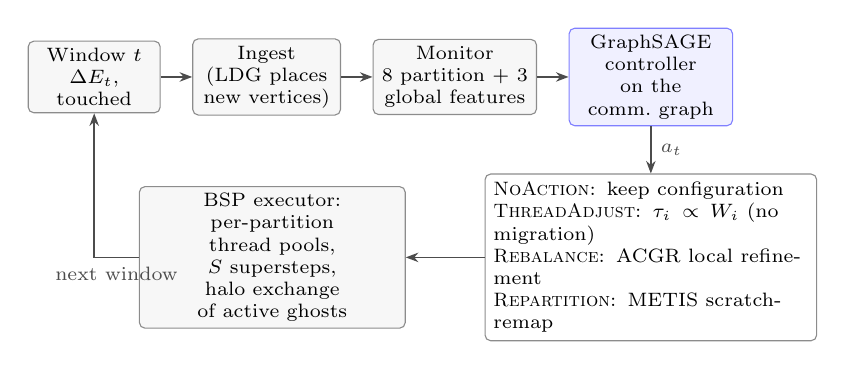
\begin{tikzpicture}[
  node distance=3.5mm and 4mm,
  box/.style={draw=black!45, rounded corners=2pt, align=center, font=\scriptsize,
              minimum height=8.5mm, inner sep=2.5pt, fill=black!3},
  act/.style={draw=black!45, rounded corners=2pt, align=left, font=\scriptsize, inner sep=3pt, fill=white},
  arr/.style={-{Stealth[length=1.6mm]}, black!70, semithick}]
  \node[box, text width=15mm] (stream) {Window $t$\\$\Delta E_t$, touched};
  \node[box, right=of stream, text width=17mm] (ingest) {Ingest\\(LDG places\\new vertices)};
  \node[box, right=of ingest, text width=19mm] (monitor) {Monitor\\8 partition + 3\\global features};
  \node[box, right=of monitor, text width=19mm, fill=blue!6, draw=blue!50] (ctrl) {GraphSAGE\\controller on the\\comm.\ graph};
  \node[act, below=6mm of ctrl, text width=40mm] (acts) {%
    \NOA{}: keep configuration\\
    \TA{}: $\tau_i \propto W_i$ (no migration)\\
    \RB{}: ACGR local refinement\\
    \RP{}: METIS scratch-remap};
  \node[box, left=10mm of acts, text width=32mm] (exec) {BSP executor: per-partition\\thread pools, $S$ supersteps,\\halo exchange of active ghosts};
  \draw[arr] (stream) -- (ingest);
  \draw[arr] (ingest) -- (monitor);
  \draw[arr] (monitor) -- (ctrl);
  \draw[arr] (ctrl) -- node[right, font=\scriptsize] {$a_t$} (acts);
  \draw[arr] (acts) -- (exec);
  \draw[arr] (exec.west) -| node[pos=0.25, below, font=\scriptsize] {next window} (stream.south);
\end{tikzpicture}
\caption{Adaptation loop of GNN-AdaptGraph. Each window is ingested, monitored and
classified by the controller. The chosen action is applied before the window is executed.}
\label{fig:arch}
\end{figure}

\subsection{Runtime State}
The state is the \emph{communication graph} of the current partitioning: one node per
partition, and an edge between two partitions that share cut edges. Each node $i$ carries
eight scale-free features:
\begin{enumerate}
  \item load share $W_i/\bar W$;
  \item thread pressure $(W_i/\tau_i)/\overline{(W/\tau)}$;
  \item ghost ratio $g_i/|P_i|$;
  \item cut ratio $c_i/e_i$;
  \item cut drift $c_i/e_i-c^0_i$ since the last (re)partitioning;
  \item load volatility $|W_i/\bar W-(W_i/\bar W)_{t-1}|$;
  \item size share $|P_i|k/|V|$;
  \item active fraction $|P_i\cap A_t|/|P_i|$.
\end{enumerate}
Here $g_i$ is the number of ghosts held by $P_i$, $c_i$ the number of its cut edges and $e_i$
the number of its incident edges. (The unnormalised features of our first version did not
generalise across graph sizes.) Three global features are broadcast to every node: the work
scale $\log_{10}(1+\sum_i W_i)/7$, the fraction of the window spent communicating, and
$\log_{10}(1+10^3 T_{\mathrm{window}})/4$. They tell the controller how much time is at stake
and whether the platform is compute-bound or communication-bound.

\subsection{GraphSAGE Controller}
The controller $f_\theta$ applies two GraphSAGE layers \cite{hamilton2017graphsage} with the
mean aggregator,
\begin{equation}
  h^{(l)}_{\mathcal{N}(i)} = \tfrac{1}{|\mathcal{N}(i)|}\textstyle\sum_{j\in\mathcal{N}(i)} h^{(l-1)}_j, \qquad
  h^{(l)}_i = \sigma\big(W^{(l)}[\,h^{(l-1)}_i \,\Vert\, h^{(l)}_{\mathcal{N}(i)}\,]\big),
\end{equation}
over the communication graph (input dimension 11, hidden dimension 64, batch normalisation,
a residual connection between the layers). A mean$\Vert$max readout pools the partition
embeddings into a graph embedding $z_t$, and an MLP ($128\!\to\!32\!\to\!4$, dropout 0.3) outputs
one logit per action: $a_t=\arg\max_a f_\theta(z_t)_a$. The model has 14{,}244 parameters.
As an ablation we replace the GraphSAGE layers with per-partition linear layers (MLP
controller, 9{,}444 parameters). This isolates the contribution of neighbourhood aggregation.

\subsection{Outcome-Based Labels and Cost-Sensitive Training}\label{sec:labels}
Our earlier controller was trained to imitate a hand-written threshold rule, so it could not
learn anything the rule did not already encode. The revised controller learns from the
\emph{outcomes} of actions. For a state at window $t$, a look-ahead oracle evaluates every
action $a\in\mathcal{A}$:
\begin{equation}\label{eq:oracle}
  J_H(a) = T^{\mathrm{adapt}}(a)+T^{\mathrm{mig}}(a) + \sum_{h=0}^{H-1} \hat T_{t+h}\big(\text{$a$ at $t$, \NOA{} afterwards}\big),
\end{equation}
where $\hat T$ is the predicted window time (execution plus network) and $H=8$. The label is
$a^\star_t=\arg\min_a J_H(a)$. Because the graph stream does not depend on the actions, the
look-ahead replays exactly the windows that will follow. $\hat T$ comes from a cost model
calibrated on the real executor (Sect.~\ref{sec:executor}):
\begin{equation}\label{eq:cost}
  \hat T^{\mathrm{exec}} = S\big(c_0 + c_1 \max_i W_i/s(\tau_i) + c_2\,\mathrm{CV}_A\big),
\end{equation}
where $s(\tau)$ is the measured parallel speedup with $\tau$ threads. Every sample stores
$J_H(a)$ for all four actions, so we train with the expected regret of the predicted action
distribution, which is the quantity the system cares about:
\begin{equation}\label{eq:loss}
  \mathcal{L}(\theta) = \mathbb{E}_{s}\Big[\textstyle\sum_{a} \pi_\theta(a\,|\,s)\,\big(J_H(a)/J_H(a^\star)-1\big)\Big]
  + 0.1\,\mathrm{CE}\big(\pi_\theta(\cdot\,|\,s), a^\star\big).
\end{equation}
Cross-entropy treats all errors alike, although their costs differ by orders of magnitude.
Triggering METIS when \NOA{} would have been best costs far more than the reverse mistake.
Loss~\eqref{eq:loss} optimises the decision cost directly. In our data, class-weighted
cross-entropy reaches a similar test regret ($\CEregret\pm\CEregretStd$\% vs.\
$\GSregret\pm\GSregretStd$\%, Sect.~\ref{sec:results}). Training states come from an $\varepsilon$-greedy oracle behaviour policy
($\varepsilon=0.3$), so that states off the oracle's path are also covered.

\subsection{ACGR: Communication-Aware Adaptive Graph Repartitioning}\label{sec:acgr}
ACGR repairs an existing partitioning locally by migrating boundary vertices. It minimises
\begin{equation}\label{eq:acgr}
  C = \alpha\,\frac{\mathrm{cut}}{|E|} + \beta\,\frac{\mathrm{CV}}{2|E|}
    + \gamma\,\max\!\big(0,\ \lambda-\epsilon\big) + \delta\,\frac{\min(\bar s,10)}{10},
  \qquad \lambda=\frac{\max_i W_i}{\bar W}-1,
\end{equation}
where $\bar s$ is the mean absolute degree skewness of the partitions and
$(\alpha,\beta,\gamma,\delta)=(0.45,0.35,0.15,0.05)$. Every term is a cost normalised to $[0,1]$,
so lower is better. Our first version gained only one edge on Cora, and two changes fix this.
First, the communication term now uses CV~\eqref{eq:cv}. The old boundary-edge count is
exactly twice the cut, so it merely duplicated the $\alpha$ term. Second, imbalance within the
tolerance $\epsilon$ is a \emph{constraint} rather than a cost, as in METIS. Penalising every
imbalance made each move away from a balanced start look worse. A move $v: P_s\to P_t$ is
therefore admissible only if
\begin{equation}\label{eq:constraint}
  W_t + w_v \le (1+\epsilon)\,\bar W \quad\text{or}\quad W_t+w_v < W_s ,
\end{equation}
and it is accepted only if it strictly decreases $C$.

ACGR keeps, for every vertex, the number of its neighbours in each partition. A move's
change in cut and CV then costs $O(\deg v)$ to evaluate. Its change in imbalance and skew costs
$O(k)$, because the loads and the first three degree moments are kept per partition. Each pass
sorts the boundary vertices by the objective change of their best admissible move. It then
re-evaluates each move against the current state and applies it if it still improves $C$.
A pass thus costs $O(|E|+|V|k)$. Passes repeat until no move improves $C$, up to 3 in the
runtime and 10 in E1. The kernels are compiled with Numba \cite{lam2015numba}. Tests check
the incremental objective against a full recomputation on 50 random graphs.

\subsection{Executor and Real Thread Adjustment}\label{sec:executor}
Each superstep runs Eq.~\eqref{eq:layer} on the active rows of every partition. A row block
is split into $\tau_i$ chunks of equal work and executed by Numba kernels that release the
Python GIL, on a thread pool dedicated to partition $i$. \TA{} therefore really changes the
parallelism of a partition: the thread pools are rebuilt with the new $\tau$ (\ReconfMs\,ms).
Exchanges copy only the values of active boundary vertices into the ghost buffers of the
receiving partitions. The executor's output matches a sequential SciPy reference to
$10^{-5}$ for any partitioning, thread allocation and active set.

\section{Experimental Setup}\label{sec:setup}

\paragraph{Hardware and software.}
All experiments run on one laptop: AMD Ryzen~5 5600H (6 cores, 12 hardware threads), 8\,GB RAM,
Windows~11. We use Python 3.12, NumPy 1.26, Numba 0.66 \cite{lam2015numba}, PyTorch 2.8, PyTorch
Geometric 2.8 \cite{fey2019pyg}, NetworkX 3.5 and METIS 5 (pymetis). The thread budget is
$T_{\mathrm{thr}}=12$, with $S=20$ supersteps per window and $F=64$. Code, seeds and the scripts
that regenerate every table and figure are released with the paper.

\paragraph{Datasets.}
Table~\ref{tab:datasets} lists the graphs. Static partition quality is measured on Cora and
PubMed \cite{sen2008collective,yang2016planetoid}, on DBLP co-authorship, and on the union of all
sx-mathoverflow edges. The dynamic experiments use two streams:
\begin{itemize}
  \item the \emph{real} temporal stream sx-mathoverflow \cite{paranjape2017motifs}, with
        \MathInteractions{} timestamped interactions (self-loops removed) over \MathYears{} years.
        The first half of the interactions builds the initial graph; the rest is split into
        30 windows. An edge expires after a quarter of the time span without interaction, so the
        graph both grows and shrinks;
  \item \emph{synthetic} streams on PubMed, driven by a Markov chain over three regimes: quiet
        (background activity only), hotspot (60\% of one community becomes active) and drift (a
        quarter of a community rewires to another one), plus preferential-attachment growth.
\end{itemize}
Neither stream, and neither of their base graphs, is used for training.

\begin{table}[t]
\centering
\caption{Graphs and streams. Dynamic streams have 30 windows; $|A_t|/|V|$ is the mean active fraction.}\label{tab:datasets}
\IfFileExists{tables/datasets.tex}{\scriptsize
\begin{tabular}{@{}lllrrrr@{}}
\toprule
Graph & Use & Type & $|V|$ & $|E|$ & avg.\ deg. & $|A_t|/|V|$ \\
\midrule
Cora & static & citation & 2,708 & 5,278 & 3.9 & -- \\
PubMed & static & citation & 19,717 & 44,324 & 4.5 & -- \\
DBLP & static & co-authorship & 4,057 & 3,528 & 1.7 & -- \\
sx-mathoverflow (all edges) & static & Q\&A & 24,759 & 187,986 & 15.2 & -- \\
sx-mathoverflow & real stream & Q\&A & 10,958$\to$24,759 & 56,928$\to$41,936 & -- & 0.49 \\
PubMed-synthetic & synth.\ stream & citation & 19,717$\to$21,556 & 44,324$\to$52,975 & -- & 0.09 \\
\bottomrule
\end{tabular}
}{\RES{table missing}}
\end{table}

\paragraph{Baselines.}
\emph{Static partitioning:} METIS \cite{karypis1998metis}, recursive Kernighan--Lin (KL)
\cite{kernighan1970}, LDG \cite{stanton2012ldg}, FENNEL \cite{tsourakakis2014fennel} and
random hashing. Each is combined with no refinement, with label-propagation refinement (LP, as
in Spinner \cite{martella2017spinner}), with ACGR, and with a cut-only ACGR ablation.
\emph{Dynamic policies:}
\begin{itemize}
  \item \emph{Static}: the initial METIS partition plus LDG placement, with no adaptation;
  \item \emph{Always-TA} and \emph{Always-ACGR};
  \item \emph{Periodic-METIS}: scratch-remap every 5 windows \cite{schloegel2000unified};
  \item \emph{Threshold}: a rule on the same features (drift $\to$ \RB{}/\RP{}, thread
        pressure $\to$ \TA{}) whose three thresholds are grid-searched on the training data;
  \item \emph{MPC}: model-predictive control with the cost model and a persistence forecast.
        The time it spends running ACGR and METIS speculatively is charged as overhead;
  \item the \emph{MLP} ablation;
  \item the look-ahead \emph{Oracle}. It sees future windows, so it is an upper bound and cannot
        be deployed.
\end{itemize}

\paragraph{Controller training.}
The training data are 450 synthetic streams of 16 windows each:
\begin{itemize}
  \item 300 \emph{regime streams} on stochastic block models, Holme--Kim power-law cluster
        graphs, random geometric graphs and Watts--Strogatz graphs with 3k--25k vertices;
  \item 150 \emph{interaction streams} from a generative model of growing interaction graphs.
        New vertices join topics whose popularity drifts. Interactions follow
        recency-weighted preferential attachment, triadic closure and topic homophily. The
        events are windowed with edge expiry exactly like the real stream.
\end{itemize}
In a first iteration we trained on regime streams only, and the controller never learned to
repartition: steady, growth-driven drift, which is typical of interaction graphs, was absent
from that data. We therefore added the second family. Its generator follows general properties
of temporal networks and was not fitted to sx-mathoverflow. The first-iteration results are
kept in the artefact.

Platform (SM, 10\,GbE, 1\,GbE), $k\in\{4,8\}$ and the stream parameters are randomised.
Samples are split 70/15/15 \emph{by stream}. Training uses AdamW (learning rate $10^{-3}$,
weight decay $10^{-4}$), batch size 64 and loss~\eqref{eq:loss}, reduces the learning rate on
plateaus (factor 0.5, patience 10), and stops early on validation regret (patience 30, at most
300 epochs). Each controller is trained with three seeds. E3 uses the seed-0 models, fixed
before evaluation.

\paragraph{Protocol and statistics.}
For each stream, $k\in\{4,8\}$ and platform, every policy first runs through the stream, and
its decisions and overheads are recorded. Then, for every window, each distinct configuration
(assignment and threads) is executed 10 times on the real executor, with policies interleaved
in random order. A window's execution time is the median of its 10 repetitions, because the
8\,GB machine occasionally stalls a run through paging. We report the number of outlier runs,
i.e.\ runs taking more than three times the window median. $J$~\eqref{eq:J} sums over windows.
Its 95\% CI is obtained by bootstrapping the repetitions of each window (1{,}000 resamples), and
synthetic streams are averaged over 3 seeds. Significance against Static is tested with a
paired Wilcoxon signed-rank test on per-window times.

\section{Results}\label{sec:results}

\subsection{Executor and Cost Model (E4)}
Thread adjustment acts on real parallelism. One partition reaches a speedup of \SpeedupSix{}
on the 6 physical cores and \SpeedupMax{} at \SpeedupMaxThreads{} threads, with no further
gain from simultaneous multithreading (\SpeedupTwelve{} at 12 threads). The cost
model~\eqref{eq:cost}, fitted on \CalPoints{} measured configurations, predicts held-out
configurations with $R^2=\CalRtwo$ and a mean absolute percentage error of \CalMape\%. This is
accurate enough to rank actions for the oracle labels. All headline results below use measured
time, not the model. The speedup curve and the fit are plotted in the artefact.


\subsection{Static Partition Quality (E1)}
Table~\ref{tab:e1} separates ACGR's contribution from that of the initial partitioner.
\begin{itemize}
  \item \emph{Repairing degraded partitions.} A partitioning that has absorbed many updates
        resembles a streaming (LDG) one. From LDG starts, ACGR reduces the edge cut by
        \EOnePubLDGCutRed\% on PubMed and \EOneCoraLDGCutRed\% on Cora (LP:
        \EOnePubLDGLPRed\% and \EOneCoraLDGLPRed\%). It obtains the lowest cut and CV of all
        refiners on the sparse graphs while staying within the 3\% balance tolerance.
  \item \emph{The CV term matters.} The cut-only ablation is no better than LP. The full
        objective lowers both CV and the cut.
  \item \emph{From METIS starts,} ACGR mainly trades cut for communication: CV falls by
        \EOnePubMetisCVRed\% on PubMed (cut change \EOnePubMetisCutRed\%).
  \item \emph{Limits.} METIS from scratch remains far better and is fast (\EOnePubMetisMs\,ms on
        PubMed). On the dense, power-law sx-mathoverflow graph, all local refiners gain little
        (\EOneMathLDGCutRed\% for ACGR from LDG). ACGR takes \EOnePubAcgrMs\,ms (PubMed, $k=8$),
        more than LP but small compared with an execution window.
\end{itemize}
Our first version reported a one-edge gain on Cora (744$\to$743). Its ACGR started from
Kernighan--Lin and penalised every imbalance. With the balance constraint and the CV term,
the same start yields the KL/ACGR rows of Table~\ref{tab:e1}.

\begin{table}[t]
\centering
\caption{Static partition quality, $k=8$, mean over 5 seeds: edge cut (\% of $|E|$),
communication volume (CV) and refinement time (ms).}\label{tab:e1}
\IfFileExists{tables/e1_quality_k8.tex}{\resizebox{\linewidth}{!}{\begin{tabular}{llrrrrrrrrrrrr}
\toprule
Initial & Refiner & \multicolumn{3}{c}{cora} & \multicolumn{3}{c}{pubmed} & \multicolumn{3}{c}{dblp} & \multicolumn{3}{c}{sx-mathoverflow} \\
 & & cut \% & CV & ms & cut \% & CV & ms & cut \% & CV & ms & cut \% & CV & ms \\
\midrule
METIS & none & 10.4 & 818 & -- & 11.8 & 6251 & -- & 5.7 & 280 & -- & 46.7 & 35839 & -- \\
METIS & LP & 10.2 & 812 & 0.7 & 11.7 & 6241 & 7.1 & 5.6 & 280 & 0.6 & 45.6 & 33932 & 10.8 \\
METIS & ACGR-cut & 10.2 & 812 & 1.6 & 11.7 & 6241 & 15.9 & 5.6 & 280 & 0.5 & 44.7 & 33440 & 87.2 \\
METIS & ACGR & 10.2 & 786 & 1.9 & 11.8 & 5994 & 22.5 & 5.6 & 274 & 0.9 & 44.9 & 33165 & 121.5 \\
\addlinespace
KL & none & 20.3 & 1626 & -- & 24.0 & 13114 & -- & 15.9 & 831 & -- & -- & -- & -- \\
KL & LP & 20.2 & 1615 & 0.7 & 23.3 & 12763 & 8.3 & 15.8 & 829 & 0.6 & -- & -- & -- \\
KL & ACGR-cut & 20.2 & 1615 & 2.2 & 23.3 & 12756 & 44.8 & 15.8 & 829 & 1.2 & -- & -- & -- \\
KL & ACGR & 19.8 & 1524 & 5.0 & 22.9 & 11958 & 55.9 & 15.3 & 790 & 2.6 & -- & -- & -- \\
\addlinespace
LDG & none & 38.7 & 2947 & -- & 45.7 & 24888 & -- & 30.4 & 1609 & -- & 74.4 & 56707 & -- \\
LDG & LP & 28.7 & 2255 & 0.9 & 30.9 & 16933 & 16.0 & 21.0 & 1101 & 0.8 & 72.4 & 54039 & 13.1 \\
LDG & ACGR-cut & 28.3 & 2239 & 6.8 & 30.5 & 16843 & 86.6 & 20.9 & 1102 & 3.2 & 72.6 & 54021 & 117.4 \\
LDG & ACGR & 24.5 & 1833 & 8.6 & 27.0 & 14249 & 97.4 & 18.3 & 927 & 3.8 & 72.8 & 53893 & 96.7 \\
\addlinespace
\bottomrule
\end{tabular}
}}{\RES{table missing}}
\end{table}

\subsection{Controller Quality (E2)}
The \NumSamples{} labelled states split into \LabelNO\% \NOA{}, \LabelTA\% \TA{}, \LabelRB\%
\RB{} and \LabelRP\% \RP{}. Table~\ref{tab:e2} reports decision quality on the
\NumTest{} test states from \NumTestGraphs{} unseen streams.
\begin{itemize}
  \item \emph{Learned versus rule-based.} The learned controllers reduce regret by about a
        quarter compared with the tuned threshold rule: GraphSAGE $\GSregret\pm\GSregretStd$\%,
        MLP $\MLPregret\pm\MLPregretStd$\%, threshold \THregret\%, never adapting \NOregret\%,
        always adjusting threads \TAallregret\%. Their macro-F1 is also higher (\GSFOne{} vs.\
        \THFOne). Always rebalancing (\RBallregret\%) or repartitioning (\RPallregret\%) is far
        worse, so firing the expensive actions at the wrong time is costly.
  \item \emph{What is learned.} Grid search sets the threshold rule's drift threshold to
        $\infty$, so it never rebalances. The GraphSAGE controller selects \RB{} in \GSPredRB\%
        of the states, with \GSRBprec\% precision and \GSRBrecall\% recall (Fig.~\ref{fig:e2}a).
        It never selects \RP{}: in \GSRPasRB\% of the states where global repartitioning is
        optimal, it chooses the cheaper local repair instead, which is a conservative choice
        given that a mistaken \RP{} costs \RPallregret\% on average. In the first iteration,
        trained without interaction streams, the controller selected neither \RB{} nor \RP{}
        (Sect.~\ref{sec:setup}). Selecting \RB{} on synthetic test states does not yet carry over
        to the real stream (E3).
  \item \emph{Ablations.} Message passing helps little: GraphSAGE and the MLP reach the same
        regret. With $k\le 8$, the communication graph is small and nearly complete, so pooling
        already exposes most of the information. Class-weighted cross-entropy performs
        similarly to the cost-sensitive loss ($\CEregret\pm\CEregretStd$\%).
\end{itemize}

\begin{figure}[t]
\centering
\IfFileExists{figs/e2_controller.pdf}{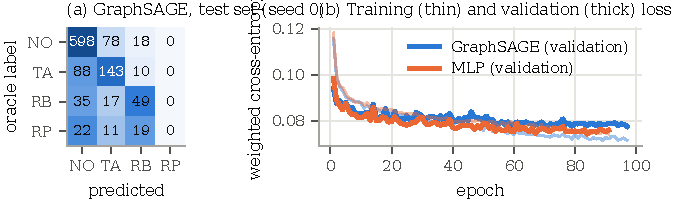
\includegraphics[width=\linewidth]{figs/e2_controller.pdf}}{\RES{figure missing}}
\caption{(a) Test confusion matrix of the GraphSAGE controller (NO: \NOA{}, TA: \TA{}, RB:
\RB{}, RP: \RP{}). (b) Loss curves of GraphSAGE and MLP (seed 0).}\label{fig:e2}
\end{figure}

\begin{table}[t]
\centering
\caption{Decision quality on held-out test graphs (mean $\pm$ std over 3 seeds). Regret is the
extra look-ahead cost $J_H(a)/J_H(a^\star)-1$ of the chosen action. Cost ratio is
$\sum J_H(a)/\sum J_H(a^\star)$.}\label{tab:e2}
\scriptsize
\IfFileExists{tables/e2_controller.tex}{\begin{tabular}{lcccc}
\toprule
Controller & Accuracy & Macro-F1 & Regret (\%) & Cost ratio \\
\midrule
GraphSAGE & 0.720 $\pm$ 0.011 & 0.469 $\pm$ 0.009 & 0.69 $\pm$ 0.07 & 1.0058 \\
MLP & 0.720 $\pm$ 0.002 & 0.453 $\pm$ 0.007 & 0.69 $\pm$ 0.02 & 1.0060 \\
Threshold (tuned) & 0.658 & 0.312 & 0.91 & 1.0079 \\
Never adapt & 0.638 & 0.195 & 1.20 & 1.0091 \\
Always \TA{} & 0.222 & 0.091 & 1.16 & 1.0086 \\
Always \RB{} & 0.093 & 0.042 & 8.51 & 1.0355 \\
Always \RP{} & 0.048 & 0.023 & 17.93 & 1.0859 \\
\bottomrule
\end{tabular}
}{\RES{table missing}}
\end{table}

\subsection{End-to-End Performance on Dynamic Graphs (E3)}
Table~\ref{tab:e3} reports measured end-to-end times on \NumScenarios{} scenarios
(2 streams $\times$ 2 values of $k$ $\times$ 3 platforms).
\begin{enumerate}
  \item \emph{Which adaptation pays depends on the workload.} On the hotspot-driven PubMed
        streams, thread reallocation gives the largest gains: Always-\TA{} is up to
        \SpPubEightSmAlwaysTA$\times$ faster than Static ($k=8$, SM), whereas periodic METIS is
        slower than Static (\SpPubEightSmPMETIS$\times$) because it migrates many vertices for
        little structural gain. On the steadily drifting real stream, periodic global
        repartitioning is the best deployable policy (\SpMathFourOnePMETIS$\times$ at $k=4$ on
        1\,GbE; Oracle \SpMathFourOneOracle$\times$), and thread reallocation adds little
        (\SpMathFourOneAlwaysTA$\times$).
  \item \emph{The learned controllers perform on par with simple heuristics, not better.}
        No fixed heuristic is best everywhere: periodic METIS is up to \RobPMETISMax\% and
        Always-\TA{} up to \RobAlwaysTAMax\% behind the best deployable policy of a scenario.
        GraphSAGE is behind by \RobGSAGEMean\% on average (worst case \RobGSAGEMax\%), slightly
        more than Always-\TA{} (\RobAlwaysTAMean\%) and the threshold rule
        (\RobThresholdMean\%), and similar to the MLP (\RobMLPMean\%). It beats Static in
        \FasterGSAGE{} of the \NumScenarios{} scenarios, significantly in \SigFasterGSAGE{}. On
        the real stream at $k=8$, all thread-adjusting policies are marginally slower than
        Static. Its controller overhead is \CtrlGSAGE\% of the total time, and it is not the
        best policy in any scenario.
  \item \emph{The gap to the Oracle is global repartitioning.} On sx-mathoverflow the Oracle
        chooses \RB{} \MathRBOracle{} times and \RP{} \MathRPOracle{} times. The learned
        controllers trigger neither action on the evaluation streams, although they select \RB{}
        on synthetic test states (E2).
  \item \emph{Speculative or unconditional repartitioning does not pay.} MPC must run ACGR and
        METIS in every window to evaluate them, and is slower than Static in every scenario
        (e.g.\ \SpPubEightSmMPC$\times$). This is the main argument for a millisecond-scale
        learned or rule-based trigger. Always-ACGR is slower than Static except on the real
        stream with $k=4$ on 1\,GbE (\SpMathFourOneAlwaysACGR$\times$).
\end{enumerate}

\begin{table}[t]
\centering
\caption{End-to-end time $J$ (s): sum of per-window median times plus overheads (mean over
seeds for PubMed). Bold: best deployable policy. $^{*}$: $p<0.05$ versus Static (paired
Wilcoxon on per-window times, all seeds).}\label{tab:e3}
\IfFileExists{tables/e3_totals.tex}{\resizebox{\linewidth}{!}{\begin{tabular}{lllrrrrrrrrr}
\toprule
Stream & $k$ & Platform & Static & Always-TA & Always-ACGR & P-METIS & Threshold & MPC & MLP & GraphSAGE & Oracle \\
\midrule
PubMed-synthetic & 4 & sm & 1.05 & \textbf{0.97} & 1.34$^{*}$ & 1.21 & 0.98 & 3.24$^{*}$ & 1.00 & 1.00 & 1.02 \\
PubMed-synthetic & 4 & 10g & 1.54 & \textbf{1.46} & 1.86$^{*}$ & 1.71 & 1.47 & 3.70$^{*}$ & 1.49 & 1.49 & 1.52 \\
PubMed-synthetic & 4 & 1g & 3.12 & \textbf{3.04} & 3.75$^{*}$ & 3.51 & 3.05 & 5.59$^{*}$ & 3.08 & 3.08 & 2.99$^{*}$ \\
PubMed-synthetic & 8 & sm & 1.33 & \textbf{1.07}$^{*}$ & 1.57 & 1.61 & 1.08$^{*}$ & 3.80$^{*}$ & 1.11 & 1.11 & 1.10$^{*}$ \\
PubMed-synthetic & 8 & 10g & 3.26 & \textbf{3.00}$^{*}$ & 3.49 & 3.54 & 3.02$^{*}$ & 5.74$^{*}$ & 3.03$^{*}$ & 3.04$^{*}$ & 3.03$^{*}$ \\
PubMed-synthetic & 8 & 1g & 7.20 & \textbf{6.94}$^{*}$ & 7.50$^{*}$ & 7.54 & 6.95$^{*}$ & 9.60$^{*}$ & 6.96$^{*}$ & 6.97$^{*}$ & 6.81$^{*}$ \\
sx-mathoverflow & 4 & sm & 4.44 & 4.15$^{*}$ & 4.61$^{*}$ & \textbf{3.93}$^{*}$ & 4.17$^{*}$ & 7.11$^{*}$ & 4.20$^{*}$ & 4.28$^{*}$ & 3.88$^{*}$ \\
sx-mathoverflow & 4 & 10g & 6.04 & 5.75$^{*}$ & 6.19$^{*}$ & \textbf{5.39}$^{*}$ & 5.78$^{*}$ & 8.17$^{*}$ & 5.80$^{*}$ & 5.80$^{*}$ & 5.35$^{*}$ \\
sx-mathoverflow & 4 & 1g & 17.56 & 17.27$^{*}$ & 16.99$^{*}$ & \textbf{15.61}$^{*}$ & 17.30$^{*}$ & 18.08 & 17.31$^{*}$ & 17.32$^{*}$ & 15.15$^{*}$ \\
sx-mathoverflow & 8 & sm & 4.93 & 5.01$^{*}$ & 5.91$^{*}$ & \textbf{4.79} & 4.98 & 8.33$^{*}$ & 4.99 & 5.00 & 4.80$^{*}$ \\
sx-mathoverflow & 8 & 10g & 8.53 & 8.61$^{*}$ & 9.55$^{*}$ & \textbf{8.31} & 8.57 & 12.03$^{*}$ & 8.58 & 8.59 & 8.26$^{*}$ \\
sx-mathoverflow & 8 & 1g & 27.46 & 27.54$^{*}$ & 28.60$^{*}$ & \textbf{26.27}$^{*}$ & 27.50 & 29.18$^{*}$ & 27.53 & 27.53 & 25.59$^{*}$ \\
\bottomrule
\end{tabular}
}}{\RES{table missing}}
\end{table}

\subsection{Discussion and Recommendations}
\begin{itemize}
  \item \emph{Transient imbalance} (hotspots) is best handled by thread reallocation. It
        costs about a millisecond, migrates nothing, and should be applied whenever thread
        pressure is uneven. Learned and rule-based triggers both do this reliably.
  \item \emph{Persistent structural drift} requires repartitioning. ACGR repairs sparse graphs
        cheaply (E1). On the dense real stream only global repartitioning helps, and it pays off
        on all three platforms.
  \item \emph{Learned control} has the lowest per-decision regret, but end to end it matches
        simple heuristics and does not exploit repartitioning on the evaluation streams. Our
        practical recommendation is a cheap thread-adjustment trigger combined with periodic or
        drift-triggered global repartitioning. Learning \emph{when to repartition globally}
        remains open: on the real stream GraphSAGE is up to \RobOracleGap\% slower than the
        Oracle.
\end{itemize}
\paragraph{Limitations.} We measure on one 6-core laptop and emulate networks analytically.
The cost model must be recalibrated for each machine, and the look-ahead assumes \NOA{} after
the first action. The dynamic experiments use one real temporal graph and $k\le 8$.

\section{Conclusion}
We revised GNN-AdaptGraph into a cost-explicit adaptive runtime for partition-parallel
processing of dynamic graphs and evaluated it on real execution with established baselines.
Thread reallocation, implemented for real, is the most effective adaptation for
activity-driven imbalance. ACGR, with a communication-volume objective and an explicit balance
constraint, repairs degraded partitions far better than label propagation on sparse graphs.
A GraphSAGE controller trained on outcome-based labels makes better per-decision choices than
a tuned rule. End to end, however, it performs on par with simple heuristics. In particular,
it does not learn when global repartitioning pays off under steady drift, where periodic
METIS remains best. The honest takeaway is a hybrid: a cheap thread-adjustment trigger
combined with drift-triggered global repartitioning. Learning the latter reliably is
the open problem.

Future work will address this gap with longer-horizon objectives (e.g.\ reinforcement
learning over whole streams), training on recorded traces of the target workload, and features
that estimate the benefit of repartitioning cheaply. We will also evaluate on a real
distributed cluster with larger graphs.


\bibliographystyle{splncs04}
\bibliography{refs}

\end{document}
